\section{Aufbau der Einzelbauteile}
Die drei Kriterien, die die Unterteilung des Modells einhalten sollen, sind wie folgt festgelegt:\\
\begin{itemize}
	\item Die Einzelteile sollen möglichst simpel gestaltet sein, um unnötig komplizierten Konflikten
	\item Die Untereinheiten sollen durch so geringe Modifikation wie möglich einen guten seitlichen Einblick in das Modell gewähren
	\item Die Untereinheiten sollen auch nach dem Entfernen einzelner Bauteile des Einblickes willen eine möglichst stabile Einheit bilden
\end{itemize}
Aus diesen Kriterien resultiert die Verwendung von herausnehmbaren Wandstücken, welche nicht zu fest im restlichen Modell verankert sind, so dass sie sehr leicht herausgenommen und auch wieder hineingesetzt werden können.
Um diese Wände auch weiterhin im Modell fixieren zu können, werden Eckpfeiler verwendet, in welche die Wandstücke, eingesetzt werden.
Da die Einheit aus Eckpfeilern und leicht entfernbaren Wandstücken nicht sehr stabil ist, werden nun am unteren Teil der Eckpfeiler noch Stecker hinzugefügt, um eine Grundplatte zu fixieren und so eine stabile Einheit zu erhalten. Zur Realisierung des Stecksystems müssen anschließend für beide Verankerungsmechanismen geeignete Designs ausgearbeitet werden.
\subsection{$\varepsilon$ Abstand}
Aufgrund des Fehlers der beim Druckprozess entsteht, wird ein Abstand zwischen den positiven und negativen definiert. \todo{Params?}


\subsection{OpenSCAD Java Interface}
Für die erleichterte Erstellung von OpenScad Objekten wurde ein Java Interface \icode{ScadObject} erstellt, welches alle für das Projekt wichtigen Befehle enthält.
Die Methode \icode{toString()} stellt in den Klassen des Interfaces die Übergabe des OpenSCAD Befehlsstrings dar.
So kann man z.B. mit der Klasse \icode{Cube} einen Quader mit Länge, Höhe und Breite erstellen der dann wie folgt mit \icode{Cube.toString()} in einen String konvertiert wird:\\
\icode{cube([Länge, Breite, Höhe]);}\\
\begin{Bild}{Ergebnis von \icode{new Cube(3, 4, 5).toString()}}
	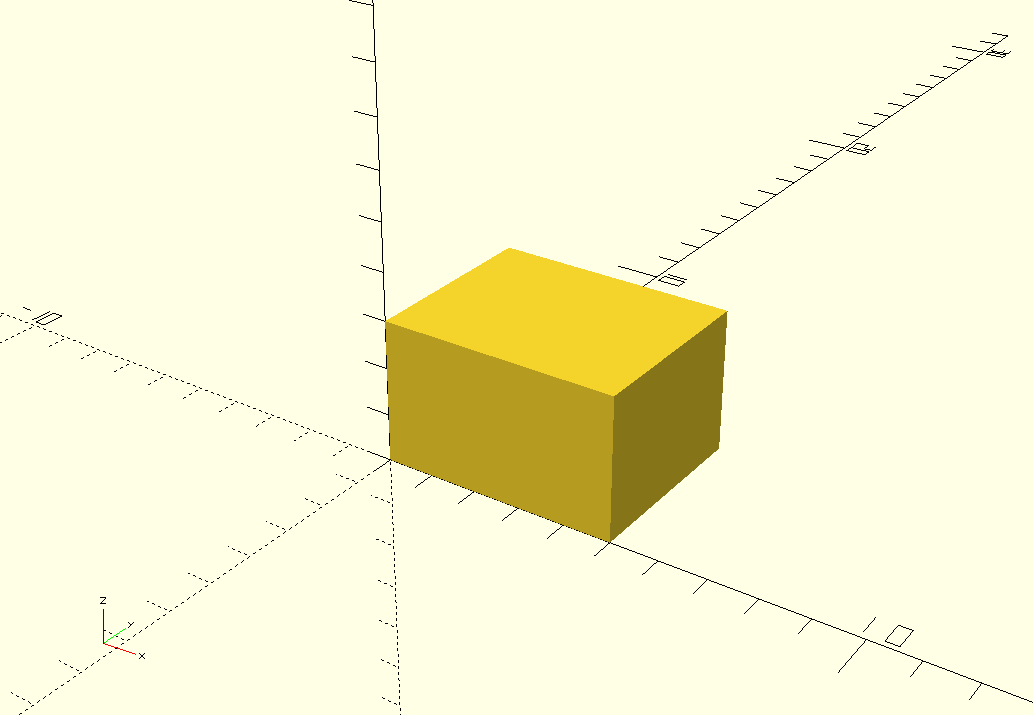
\includegraphics[width = 120mm]{Bilder/Quader}
\end{Bild}



\subsection{Corner}
Das Corner Element bezeichnet die Eckpfeiler des 3D-Modells.
Es besteht aus zwei zusammengefügten Teilen, dem CornerCylinder und dem CornerPin.
CornerCylinder stellt den oberen Teil einer Ecke dar, der ein rundes Grundbauteil mit Einkerbungen für Wände bereitstellt.
In dessen Berechnung werden alle an dem Knoten anliegenden Kanten betrachtet und eine Schnittmenge zwischen einem Grundzylinder und in die Richtung der Kanten gedrehten Quadern vollzogen.\\
\todoinline{CornerPin}
\subsection{Wall}
\subsection{BasePlate}